\section{Technology}\label{sec:tech}

  Various technologies will be used to develop OpenDCS, this section is intended
  to provide some common terms and expressions used throughout the document.

  \subsection{ZeroMQ}\label{sec:tech-zmq}

    ZeroMQ is a library that provides a means of creating systems that have
    distributed messaging. From the website (\url{http://zeromq.com}) it offers
    the ability to:

    \begin{itemize}
      \item Connect your code in any language, on any platform.
      \item Carries messages across inproc, IPC, TCP, TIPC, multicast.
      \item Smart patterns like pub-sub, push-pull, and router-dealer.
      \item High-speed asynchronous I/O engines, in a tiny library.
      \item Backed by a large and active open source community.
      \item Supports every modern language and platform.
      \item Build any architecture: centralized, distributed, small, or large.
    \end{itemize}

    Socket types are available to make several patterns possible such as
    Request-Reply (REQ-REP), Publish-Subscribe (PUB-SUB), Parallel Pipelines,
    and Fair Queuing among others. OpenDCS services will initially only be
    developed to use the PUB-SUB and the REQ-REP patterns, but could eventually
    use others. The ability to extend to these others in the future was the
    reason for selecting this library over something else, such as TCP or UDP
    sockets on their own.

    \paragraph{PUB-SUB Pattern}

      With this form of messaging the publisher sends the message, and the
      subscriber receives them. Messages are meant to be characterized such
      that they be sent without any knowledge of which subscribers will receive
      them, if any at all. Messages can be filtered by the subscriber which
      allows them to receive only the subset that is desired.

      \begin{figure}[H]
        \begin{center}
          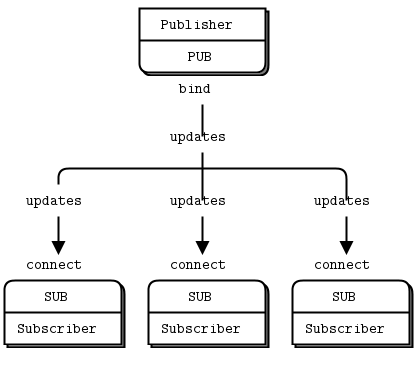
\includegraphics[width=0.5\textwidth]{figures/pub-sub-pattern}
        \end{center}
      \end{figure}

    \paragraph{REQ-REP Pattern}

      This pattern is one of the basic methods that is used in network
      application development to communicate between systems. With this type a
      connection is made and there are a series of transactions until the
      request is complete and a response is provided. A simple example of this
      is browsing a web page, a person using a web browser requests a page and
      the server responds with the page content for the browser to render

      \begin{figure}[H]
        \begin{center}
          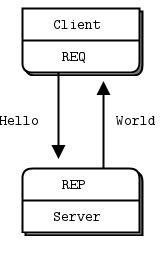
\includegraphics[width=0.25\textwidth]{figures/req-rep-pattern}
        \end{center}
      \end{figure}

  \subsection{Vala}\label{sec:tech-vala}

    Vala is a programming language that aims to bring modern programming
    language features without imposing any runtime requirements and without
    using a different ABI compared to applications and libraries written in
    C~\cite{Vala2016}.
